\documentclass[a4paper,10pt]{article}
\usepackage{luatexja}
\usepackage{luatexja-fontspec}
\usepackage{geometry}
\usepackage{multicol}
\usepackage{titlesec}
\usepackage{setspace}
\usepackage{graphicx}
\usepackage{caption}
\usepackage{indentfirst}
\usepackage{float} % 図の位置を制御するために追加
\usepackage{listings}
\usepackage{xcolor}
\usepackage{amsmath,amssymb} % align 環境などの数式用
\usepackage{hyperref}
\usepackage{physics}

\geometry{margin=20mm}
\setstretch{1.2}
\parindent=1em

% ===== 日本語フォント設定 =====
% HaranoAjiMincho がシステムに入っている必要あり
\setmainjfont{HaranoAjiMincho} % メイン日本語フォント
\setsansjfont{HaranoAjiGothic} % サンセリフ（任意）
\setmonojfont{HaranoAjiMincho} % 等幅も同じに設定（好みに応じて変更）

% 図のキャプションの表記を「図1」のように日本語化
\renewcommand{\figurename}{図}
\captionsetup[figure]{labelformat=default,labelsep=period}

\renewcommand{\tablename}{表}
\captionsetup[table]{labelformat=default,labelsep=period}

\geometry{margin=25mm}
\setstretch{1.2}
\parindent=1em

\titleformat{\section}{\large\bfseries}{\thesection.}{1em}{}

\definecolor{keywordcolor}{rgb}{0.26, 0.38, 0.68}
\definecolor{commentcolor}{rgb}{0.3, 0.6, 0.3}
\definecolor{stringcolor}{rgb}{0.7, 0.2, 0.2}

\lstdefinelanguage{SystemVerilog}{
  morekeywords={module,endmodule,input,output,logic,always_ff,if,else,begin,end,posedge,negedge},
  sensitive=true,
  morecomment=[l]{//},
  morecomment=[s]{/*}{*/},
  morestring=[b]",
}

\lstset{
  language=SystemVerilog,
  basicstyle=\ttfamily\small,
  keywordstyle=\color{keywordcolor}\bfseries,
  commentstyle=\color{commentcolor}\itshape,
  stringstyle=\color{stringcolor},
  numbers=left,
  numberstyle=\tiny,
  stepnumber=1,
  numbersep=5pt,
  frame=single,
  tabsize=2,
  showstringspaces=false,
  breaklines=true,
  breakatwhitespace=true
}

% -------------------------------------------
% Python 用の listings 言語定義
% -------------------------------------------
\lstdefinelanguage{PythonCustom}{
  language=Python,
  morekeywords={
    def,class,return,import,from,as,with,for,while,if,elif,else,
    try,except,finally,raise,pass,break,continue,lambda,yield,global,nonlocal
  },
  sensitive=true,
  morecomment=[l]{\#},
  morestring=[b]",
}

% -------------------------------------------
% Python 用スタイル
% （SystemVerilog のスタイルを完全踏襲）
% -------------------------------------------
\lstdefinestyle{pythonstyle}{
  language=PythonCustom,
  basicstyle=\ttfamily\small,
  keywordstyle=\color{keywordcolor}\bfseries,
  commentstyle=\color{commentcolor}\itshape,
  stringstyle=\color{stringcolor},
  numbers=left,
  numberstyle=\tiny,
  stepnumber=1,
  numbersep=5pt,
  frame=single,
  tabsize=2,
  showstringspaces=false,
  breaklines=true,
  breakatwhitespace=true
}

% \title{SystemVerilog Code with Listings}

\begin{document}

% タイトルブロック
\begin{center}
\noindent
{\LARGE 第5回輪講資料} \\
{\large 4321　野秋 琳太郎} \\
2025年 12月 11日
\end{center}

\begin{flushright}
指導教員　宮田 尚起
\end{flushright}    

\begin{multicols}{2}[\raggedcolumns]

\section{はじめに}
前回の進捗はKdV方程式の形をした,非線形キャパシタを想定した電信方程式の導出までであった.
しかし,非線形キャパシタで分布型定数回路を考えるならば,KdV方程式で表すよりも戸田格子としての運動方程式を考えたほうが筋が良いのではないかと思った.
今回は,戸田格子としてインダクタとバラクタダイオードを想定したLCラダー回路を考えて,ソリトン解の得られる方程式を導出する。


\section{戸田格子（Toda Lattice)}

戸田格子は,1967年に戸田盛和によって提案された,非線形相互作用を持つ1次元粒子格子のモデルである.
このモデルは,隣接する粒子間に以下の「戸田ポテンシャル」$\phi(r)$ が作用する系として定義される.

\begin{equation}
    \phi(r) = \frac{a}{b} e^{-br} + ar \quad (ab > 0)
\end{equation}

ここで,$r_n$ は第 $n$ 粒子と第 $n-1$ 粒子の相対変位（$r_n = y_n - y_{n-1}$）,$a, b$ は定数である.
このポテンシャルに対応する復元力 $f(r)$ は,ポテンシャルの空間微分として求められる.

\begin{equation}
    f(r) = -\phi'(r) = a (e^{-br} - 1)
\end{equation}

第 $n$ 粒子の質量を $m$ とすると,運動方程式は以下のように記述される.

\begin{align}
    m \frac{d^2 y_n}{dt^2} &= f(r_n) - f(r_{n+1}) \notag \\
    &= a(e^{-b(y_{n-1} - y_n)} - e^{-b(y_n - y_{n+1})})
\end{align}

あるいは,相対変位 $r_n$ の時間発展として記述する場合,上式の差分をとることで以下の戸田方程式（Toda Equation）が得られる.

\begin{align}
    m \frac{d^2 r_n}{dt^2} = a(2e^{-br_n} - e^{-br_{n-1}} - e^{-br_{n+1}})
\end{align}

この方程式は完全可積分系であり,ソリトン解（孤立波）を厳密に持つことが知られている.

\section{LCラダー回路の運動方程式の導出}

前節の力学モデルを電気回路で実現するために,図\ref{fig:lchasigo}のようなLCラダー回路を考える.
ここで,戸田格子ポテンシャルはキャパシタに蓄えられた静電エネルギー,その変数$r$はキャパシタの電荷に相当する.

\begin{figure}[H]
    \centering
    % 必要に応じて画像ファイル名を変更してください
    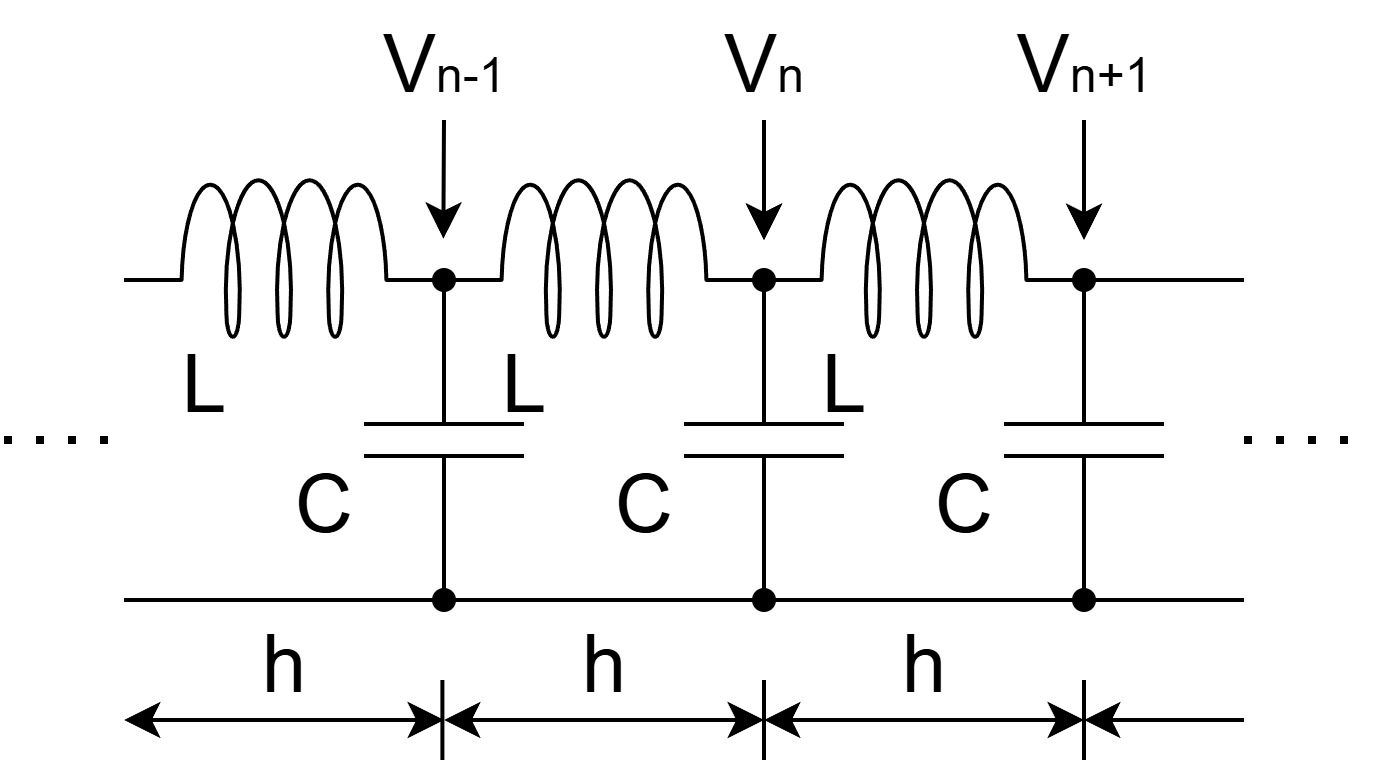
\includegraphics[width=0.8\linewidth]{figure/lchasigo.png}
    \caption{LCラダー回路の模式図}
    \label{fig:lchasigo}
\end{figure}

\subsection{キルヒホッフの法則による立式}

回路の第 $n$ セクションにおける変数を以下のように定義する.
\begin{itemize}
    \item $V_n(t)$: 第 $n$ ノードの対地電圧
    \item $I_n(t)$: 第 $n-1$ ノードから第 $n$ ノードへ向かうインダクタ電流
    \item $Q_n(t)$: 第 $n$ ノードのキャパシタに蓄えられる電荷
\end{itemize}

まず,インダクタ $L$ 両端の電位差と電流の関係（キルヒホッフの電圧則: KVL）より,以下の式が成り立つ.


\begin{equation}
    L \frac{dI_n}{dt} = V_{n-1} - V_n \label{eq:kvl}
\end{equation}

次に,ノード $n$ における電流の保存則（キルヒホッフの電流則: KCL）を考える.
ノードに流入する電流は $I_n$,流出する電流は $I_{n+1}$ であり,その差分がキャパシタへの充電電流 $\frac{dQ_n}{dt}$ となる.

\begin{equation}
    \frac{dQ_n}{dt} = I_n - I_{n+1} \label{eq:kcl}
\end{equation}

\subsection{電荷 $Q_n$ に関する方程式への変形}

式(\ref{eq:kcl})の両辺を時間 $t$ で微分する.

\begin{equation}
    \frac{d^2 Q_n}{dt^2} = \frac{dI_n}{dt} - \frac{dI_{n+1}}{dt} \label{eq:diff_kcl}
\end{equation}

ここで,式(\ref{eq:kvl})の関係を用いると,右辺の電流微分項は電圧で表現できる.
\begin{align}
    \frac{dI_n}{dt} &= \frac{1}{L}(V_{n-1} - V_n) \\
    \frac{dI_{n+1}}{dt} &= \frac{1}{L}(V_n - V_{n+1})
\end{align}

これらを式(\ref{eq:diff_kcl})に代入する.

\begin{equation}
    \frac{d^2 Q_n}{dt^2} = \frac{1}{L}(V_{n-1} - V_n) - \frac{1}{L}(V_n - V_{n+1})
\end{equation}

両辺に $L$ を掛けて整理すると,以下の回路方程式（運動方程式）が得られる.

\begin{equation}
    L \frac{d^2 Q_n}{dt^2} = V_{n-1} - 2V_n + V_{n+1} \label{eq:circuit_eom}
\end{equation}

この式は,線形・非線形を問わず,ラダー回路構造が持つ一般的な方程式である.戸田格子を実現するためには,右辺の電圧 $V$ と左辺の電荷 $Q$ の間に特定の非線形関係が必要となる.

\section{バラクタダイオードによるモデル化}

戸田格子の指数関数的な相互作用を回路で実現するために,キャパシタとしてバラクタダイオード（可変容量ダイオード）を用いる.

\subsection{バラクタダイオードの容量特性}

バラクタダイオードに逆バイアス電圧 $V_{bias}$ を印加した状態を動作点とする.信号電圧を $V$ とするとき,接合容量 $C(V)$ は一般に以下の式で近似される.

\begin{equation}
    C(V) = \frac{C_0}{(1 + \frac{V}{V_{bias}})^m}
\end{equation}

ここで $C_0$ はバイアス点での容量,$m$ は接合のプロファイルで決まる定数である.
戸田格子に対応させるため,理想的な場合として $m=1$ を仮定する（これは階段接合などで近似的に成り立つ）.

\begin{equation}
    C(V) = \frac{dQ}{dV} = \frac{C_0}{1 + \frac{V}{V_{bias}}} \label{eq:varactor_c}
\end{equation}

\subsection{電荷-電圧 ($Q-V$) 特性の導出}

式(\ref{eq:varactor_c})を変数分離して積分し,電荷 $Q$ と電圧 $V$ の関係式を求める.ただし $Q(0)=0$ とする.

\begin{align}
    dQ &= \frac{C_0}{1 + \frac{V}{V_{bias}}} dV \\
    \int_0^Q dQ' &= \int_0^V \frac{C_0 V_{bias}}{V_{bias} + V'} dV' \\
    Q &= C_0 V_{bias} \ln \left( 1 + \frac{V}{V_{bias}} \right)
\end{align}

この式を電圧 $V$ について解くと,以下の指数関数形式が得られる.
ここで,特性電荷 $Q_0 = C_0 V_{bias}$ と置いた.

\begin{equation}
    V(Q) = V_{bias} \left( e^{\frac{Q}{Q_0}} - 1 \right) \label{eq:vq_relation}
\end{equation}

\subsection{戸田格子方程式への帰着}

得られた $Q-V$ 関係式(\ref{eq:vq_relation})を,先ほど導出した回路運動方程式(\ref{eq:circuit_eom})の右辺に代入する.

\begin{equation}
    L \frac{d^2 Q_n}{dt^2} = V_{bias} \left[ \left( e^{\frac{Q_{n-1}}{Q_0}} - 1 \right) - 2\left( e^{\frac{Q_n}{Q_0}} - 1 \right) + \left( e^{\frac{Q_{n+1}}{Q_0}} - 1 \right) \right]
\end{equation}

定数項（$-1 - 2(-1) + (-1)$）は相殺されて消えるため,式は以下のように整理される.

\begin{equation}
    L \frac{d^2 Q_n}{dt^2} = V_{bias} \left( e^{\frac{Q_{n-1}}{Q_0}} - 2e^{\frac{Q_n}{Q_0}} + e^{\frac{Q_{n+1}}{Q_0}} \right)
\end{equation}



\subsection{参考文献}
\begin{itemize}
    \item 和達美樹 『岩波講座現代の物理学 非線形波動』 岩波書店 1992年
    \item pythonで学ぶ計算物理 ドキュメント » 5. 偏微分方程式 » 5.2. 【例題】KdV方程式\\ 
    \url{https://www.physics.okayama-u.ac.jp/~otsuki/lecture/CompPhys2/pde/kdv.html}\\
    (2025/11/20)
\end{itemize}

\newpage
\vfill
\end{multicols}

\end{document}
